
\chapter[Estado del Arte]{Simulación de Materiales en Computación Gráfica: Estado del Arte}
\section{Introducción} %(hablar de los diferentes materiales, cómo los modelos "fáciles" no sirven)
El renderizado en computación gráfica es el intento de producir imágenes que representan una escena tridimensional, representada por medio de primitivas matemáticas como puntos, líneas, cubos, etc.

En los últimos años, el avance en el campo del renderizado de escenas ha sido muy notorio. El nivel de realismo presente en las imágenes obtenidas ha ido en aumento hasta el punto de ser de difícil distinción para un ser humano. Dichos avances han sido, en gran parte, debido al desarrollo de dispositivos de hardware gráficos más poderosos, ya que la teoría matemática que describe el comportamiento de la luz en escenas estuvo presente desde hace varias décadas \cite{Kajiya} mediante la denominada Ecuación del Rendering.


La ecuación es una aproximación, un modelo físico que intenta describir los aspectos considerados más importantes en el fenómeno de interacción de la luz con diversos objetos en una escena.

Lamentablemente, la ecuación es, en términos teóricos, no computable. Sin embargo, el estudio a lo largo de los años de técnicas que permitan aproximarla ha dado sus frutos y ha permitido la obtención de imágenes de un realismo asombroso.

A pesar de estos increíbles avances en un corto período de tiempo, el renderizado de una escena es un problema que involucra otros inconvenientes. El más notorio de ellos, es que la ecuación del rendering no tiene en cuenta qué {\em materiales} componen los objetos que definen la escena. En otras palabras, un objeto compuesto por madera no lucirá exactamente igual que uno compuesto por metales, ni por un material orgánico compuesto de tejidos. A la par del desarrollo de técnicas de iluminación global, han surgido técnicas que han intentado abordar materiales específicos \cite{} y familias de materiales \cite{}.

Estas técnicas buscan capturar la intrincada geometría propia de cada material. Diferentes estructuras microscópicas producen distintas apariencias, reflejando la luz de distinta manera, hecho que es interpretado por la percepción humana como diferentes materiales. Por ejemplo: una superficie metálica tiene un gran componente reflexivo, emitiendo luz en direcciones bien definidas, a diferencia de una superficie más opaca como un plástico. Dado que la ecuación del rendering usa los materiales como {\em caja negra}, los mismos deben ser modelados de una manera adecuada para ser integrados en las distintas técnicas de renderizado global.

Determinados materiales han recibido mayor atención debido a su ubicuidad en escenas de películas y video juegos, o a la facilidad de su diseño: agua, fuego, aire, humo, piel humana, madera, etc. Por esta razón, las imágenes sintéticas obtenidas presentan cierta asimetría en la calidad de los distintos materiales. En contraste, otros materiales han recibido menor atención, la cual puede atribuirse a una menor presencia en escenas o a una dificultad en el modelado y visualización, la cual ha resistido las técnicas más simples.

Entre estos materiales, aquellos sometidos a un proceso de cocción han permanecido entre los más dificultosos por su compleja geometría y los fenómenos lumínicos involucrados. Tal vez el caso más emblemático de los materiales cocidos es el pan, debido a su importancia en la vida cotidiana. Como nota de color, un reconocido  científico del área, Alain Fournier, pronunció en 2001 la frase "la Computación Gráfica todavía no ha sido capaz de renderizar de manera convincente una feta de pan". En las siguientes secciones mostraremos que unos pocos intentos por abordar el problema fueron realizados pocos años después.

\section{Modelos de Geometría de Materiales}
En esta sección presentaremos distintos modelos geométricos que han hecho su aparición a lo largo de los años en computación gráfica. Los mismos son el resultado de un balance entre detalle de representación, tiempos de cómputo y recursos de memoria utilizados.

\subsection{Modelos Procedimentales}
Un modelo procedimental resulta útil en determinadas situaciones donde la supervisión humana repetitiva no es adecuada.

Existen numerosos ejemplos donde se aplica una técnica de modelado procedimental.
En las siguientes sub-secciones presentaremos los casos más comunes de aplicación, los cuales constituyen estándares actuales en el modelado de dichos materiales.


\subsubsection{Plantas}
El modelado procedimental de plantas está basado en una interpretación de una tortuga que se mueve por un plano o el espacio, construyendo la geometría de los materiales \cite{Prusinkiewicz1986}.

Las gramáticas formales \cite{Chomsky1956} intentaron describir el lenguaje natural de forma matemática, donde sub-cadenas de caracteres son reemplazadas por otras.
Siguiendo esta idea, los sistemas-L \cite{Lindenmayer1968} pretenden realizar una descripción matemática de la geometría de las plantas.
El concepto central que permite entender el modelado procedimental utilizando sistemas-L es el de {\em reescritura}.
La reescritura consiste en una aplicación sucesiva de reglas que reemplazan determinadas partes en una descripción matemática por otras.
En un sistema-L, una cadena de caracteres representa la estructura de la planta.

\paragraph{Definición de sistema-L}
Sea $V$ un alfabeto (conjunto de caracteres), $V^{*}$ el conjunto de todas las palabras que se pueden formar con $V$ y $V^{+}$ el conjunto de todas las palabras que se pueden formar y no son vacías.
Una sistema-L de cadenas es una tripleta $G = (V,\omega,P)$, donde $V$ es el alfabeto, $\omega \in V^{+}$ es una cadena no vacía llamada {\em axioma} y $P \subset V \times V^{*}$ es un conjunto finito de reglas de producción.
Una producción $(a,\chi)$ se denota $a \rightarrow \chi$.
$a$ es llamado el {\em predecesor} y $\chi$ el {\em sucesor} de la producción.
Si no se especifica ninguna producción para $a$, se asume $a \rightarrow a \in P$.

Sea $\mu = a_{1}, \dots, a_{m}$ una palabra en $V$.
Se dice que la palabra $\mu_{1}, \dots, \mu_{m}$ es {\em derivada directamente} de $\mu$, y se nota $\mu \Rightarrow \eta$,  si y sólo si $a_{i} \rightarrow \mu_{i}, \forall i = 1, \dots, m$.

Una palabra $\eta$ es generada por $G$ si existe una secuencia de cadenas que conducen a $\eta$ desde el axioma, es decir, $\mu_{1},\dots,\mu_{n}$, de tal forma que $\mu_{1} = \omega$ y $\mu_{n} = \eta$ y $\mu_{1} \Rightarrow \dots  \Rightarrow \mu_{n}$.

Un ejemplo de esto es expuesto a continuación.
Si el axioma es $\omega = a$, y las reglas de producción son:
\begin{align*}
p1 &: a \rightarrow b,\\
p2 &: b \rightarrow ab,
\end{align*}

entonces una cadena de derivaciones podría resultar $a, b, ab, bb, abab, \dots$, donde las reglas aplicadas en cada paso serían $p1, p2, p1, p2$ (dos veces).

Estos sistemas fueron diseñados buscando representar las divisiones celulares existentes en ciertas amebas.
Sin embargo, luego se mostrará que los mismos pueden ser utilizados como modelos para capturar la geometría de diversos objetos.

\paragraph{Interpretación de Tortuga}
El estado de la tortuga se define por una tripleta $(x,y,\alpha)$, donde $x,y$ representan la posición de la tortuga y $\alpha$ es el ángulo hacia donde {\em apunta} la tortuga.
Dado un tamaño de paso $d$ y un incremento angular de $\delta$, la tortuga puede "programarse" para responder a cadenas de caracteres con la siguiente interpretación,

\begin{itemize}
\item F, moverse hacia adelante un paso d, dibujando,
\item f, moverse hacia adelante un paso d, sin dibujar,
\item +, rotar un ángulo $\delta$,
\item -, rotar un ángulo $-\delta$.
\end{itemize}

Al interpretarse el comando $F$, el nuevo estado de la tortuga será $(x',y',\alpha)$, donde $x' = x + d * cos(\alpha)$ y $y' = y + d * sin(\alpha)$. Se dibuja además una línea entre $(x,y)$ y $(x',y')$.
Al interpretarse el comando $f$ ocurre lo mismo, sólo que la línea no se dibuja.
Cuando se lee el comando $+$ (girar a la izquierda). el nuevo estado pasa a ser $(x,y,\alpha-\delta)$ y cuando se interpreta $-$ (girar a la derecha),  $(x,y,\alpha+\delta)$.

De esta forma, dada una cadena $\eta$, la interpretación de tortuga de la misma es la imagen que se genera al responder la tortuga a los comandos inducidos por $\eta$.
La Fig.~\ref{fg:tortuga} muestra un ejemplo de la figura resultante de la cadena FFF-FF-F-F+F+FF-F-FFF, donde la tortuga comienza {\em mirando} hacia arriba, y $\delta = 90^{\circ}$.

\begin{figure}
\center
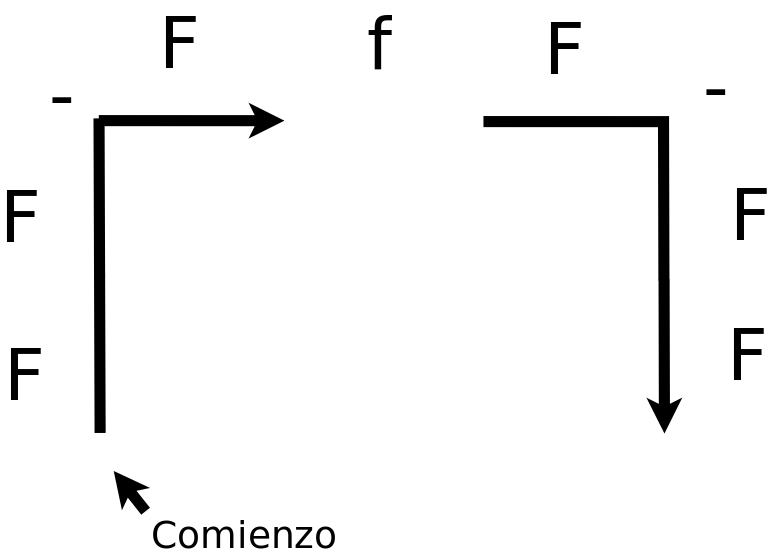
\includegraphics[width=8cm]{figures/tortuga}
\caption{Resultado de la interpretación de tortuga de una cadena de caracteres.}
\label{fg:tortuga}
\end{figure}

La Fig.~\ref{fg:tortuga} muestra otros ejemplos de sistemas-L, en los cuales se puede observar que con pocas reglas es posible obtener estructuras complejas y de gran belleza.

Usualmente, y debido a la utlización de recursión y repetición, estos sistemas dan lugar a figuras fractales, por lo cual se las utiliza para dibujar este tipo de estructuras autosimilares.

\begin{figure}
\center
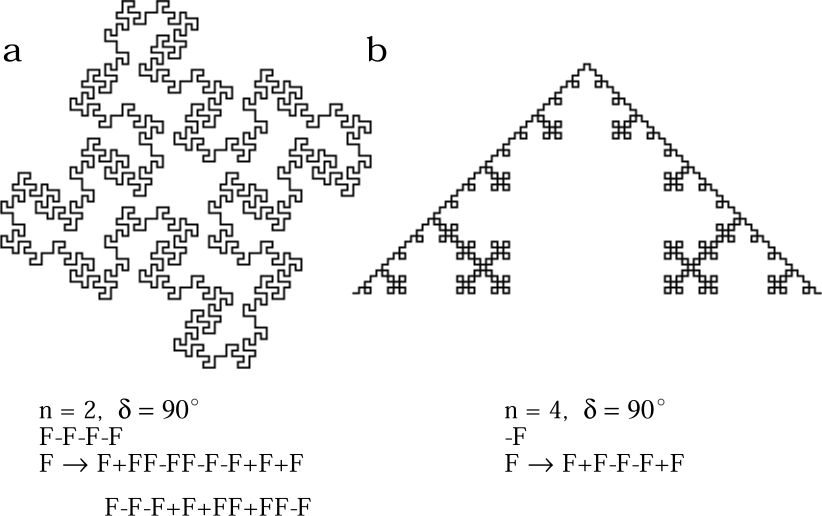
\includegraphics[width=13cm]{figures/sistemasL}
\caption{Sistemas-L generados utilizando distintos parámetros. $n$ es la cantidad de derivaciones utilizadas para producir la cadena que da origen a la figura. En (a), el axioma es F-F-F-F, mientras que en (b) es -F.}
\label{fg:sistemasL}
\end{figure}

Para lograr una imagen que semeje la estructura de árboles y plantas, es necesario introducir dos nuevos caracteres, los cuales son utilizados para generar estructuras ramificadas.
Utilizando una {\em pila} de estados, es posible alcanzar este comportamiento.
Los caracteres $[$, y $]$ se utilizan para mover el estado actual a la pila, y para reemplazar el estado actual con el de la pila, respectivamente.
El estado actual de la tortuga está representado por la tripleta antes mencionada.
Por lo tanto, al realizar la operación $]$, en general la posición y orientación de la tortuga cambiarán.
La utilización de un par $[\dots]$ produce que la tortuga dibuje una rama y vuelva al punto inicial, permitiendo continuar con la computación de otras partes de la estructura.

\begin{figure}
\center
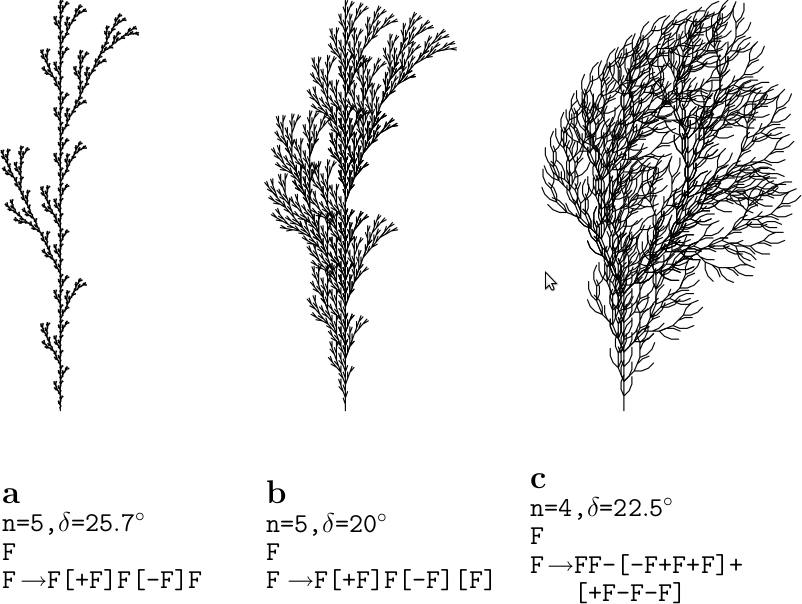
\includegraphics[width=13cm]{figures/sistemalcorchete}
\caption{Sistemas-L con pila de estados, utilizando distintos parámetros. Las imágenes muestran estructuras muy parecidas a plantas. $n$ es la cantidad de derivaciones utilizadas para producir la cadena que da origen a la figura.}
\label{fg:sistemasLcorchete}
\end{figure}

\subsubsection{Edificios y Ciudades}
\cite{Parish2001} \cite{Muller2006},
\subsubsection{Planetas}
\cite{Ebert2002}
\subsubsection{Montañas}

Existen numerosas variantes a estos sistemas, entre los cuales encontramos sistemas-L estocásticos, los cuales eligen reglas de reescritura de acuerdo a una probabilidad que se pasa como parámetro, sistemas-L paramétricos, los cuales hacen variar el ángulo y el paso a dibujar dependiendo de la posición de la cadena donde se encuentran, y muchos otros.
Además, el método es fácilmente generalizable en tres dimensiones, ver \cite{Prusinkiewicz1990} para obtener mayores detalles.

\subsection{Modelos Físicos}
Desde el surgimiento del área, estos modelos han ido evolucionando gracias al incremento en el poder de cómputo del hardware gráfico disponible. Sin embargo, aún nos encontramos en los comienzos de una aplicación más difundida de los mismos.
\subsubsection{Fluídos}
\subsubsection{Telas}

\section{Representación (Renderizado)}
\subsection{Ecuación del Rendering}

\begin{equation}
EC  = REND
\end{equation}

, donde.


\subsection{BRDFs}
\subsection{Radiancia}
\subsection{Simplificaciones}
Todas estas simplificaciones son realizadas a escala humana, es decir, sin tener en consideración la naturaleza microscópica de la luz. En esta escala, las trayectorias que describe la luz son aproximadas por líneas rectas.
\subsubsection{Ray Tracing}
\subsubsection{Radiosity}
\subsubsection{Photon Mapping}
\subsubsection{Ray Marching}
\subsubsection{Volume Rendering}

\section{Materiales específicos:}
\subsection{Agua}
\subsection{Fuego}
\subsection{Humo}
\subsection{Piel}
\subsection{Otros}


\section{Conclusiones}

